%
% Sección de cifrado por bloques, capítulo de antecedentes.
% Proyecto Lovelace.
%

\section{Cifrados por bloques}

Los cifrados por bloque son esquemas de cifrado que, como bien
lo explica su nombre, operan mediante bloques de datos. Normalmente los
bloques tienen una longitud de 64 o de 128 bits, mientras que las llaves
pueden ser de 56, 128, 192 o 256 bits.

En muchos sistemas criptográficos, los cifrados por bloque simétricos 
son elementos importantes, pues su versatilidad permite construir con 
ellos generadores de números pseudoaleatorios, cifrados de flujo MACs y
funciones hash. Sirven también como componentes centrales en técnicas de
autenticación de mensajes, mecanismos de integridad de datos, protocolos
de autenticación de entidad y esquemas de firma electrónica que usan
llaves simétricas.

Los cifrados por bloque están limitados en la práctica por varios
factores, tales como el límite de memoria, la velocidad requerida o
restricciones impuestas por el hardware o el software en el que se
implementan. Normalmente, se debe escoger entre eficiencia y seguridad

Idealmente, al cifrar por bloques, cada bit del bloque cifrado depende
de todos los bits de la llave y del texto en claro; no debería existir
una relación estadística evidente entre el texto en claro y el texto
cifrado; el alterar tan solo un bit en el texto en claro o en la llave
debería alterar cada uno de los bits del texto cifrado con una
probabilidad de $\frac{1}{2}$; y alterar un bit del texto cifrado
debería provocar resultados impredecibles al recuperar el texto en
claro.

\subsection{Definición}

\begin{equation}
  \label{cifrado_bloques_def}
  E: \{0,1\}^r \times \{0,1\}^n \longrightarrow \{0,1\}^n
     (k,m) \longmapsto  E(k,m)
\end{equation}


Utilizando una llave secreta $k$ de longitud binaria $r$ el algoritmo de
cifrado $E$ cifra bloques en claro $m$ de una longitud binaria fija $n$ y
da como resultado bloques cifrados $c = E (k,m)$ cuya longitud también es
$n$. $n$ es el tamaño de bloque del cifrado.
El espacio de llave está dado por $K = \{0,1\}^r$, para cada llave existe una 
función $D_k(c)$ que permite tomar un bloque cifrado $c$ y regresarlo a su 
forma original $m$.

Generalmente, los cifrados por bloque procesan el texto claro en bloques
relativamente grandes ($n \geq 64$), contrastando con los cifradores de
flujo, que toman bit por bit. Cuando la longitud del mensaje en claro excede 
el tamaño de bloque, se utilizan los modos de operación.

Los parámetros más importantes de los cifrados por bloque son los
siguientes:
\begin{itemize}
  \item Tamaño de bloque
  \item Tamaño de llave
\end{itemize}

\subsection{Criterios para evaluar los cifrados por bloque}

A continuación se listan algunos de los criterios que pueden ser tomados 
en cuenta para evaluar estos cifrados:
\begin{enumerate}
  \item \textbf{Nivel de seguridad.} La confianza que se le tiene a un
    cifrado va creciendo con el tiempo, pues va siendo analizado y
    sometido a pruebas.
  \item \textbf{Tamaño de llave.} La entropía del espacio de la llave
    define un límite superior en la seguridad del cifrado al tomar en
    cuenta la búsqueda exhaustiva. Sin embargo, hay que tener cuidado
    con su tamaño, pues también aumentan los costos de generación,
    transmisión, almacenamiento, etcétera.
  \item \textbf{Tamaño de bloque.} Impacta la seguridad, pues entre más
    grandes, mejor; sin embargo, tiene repercusiones en el costo de la
    implementación, además de que puede afectar el rendimiento del
    cifrado.
  \item \textbf{Expansión de datos.} Es extremadamente deseable que los
    datos cifrados no aumenten su tamaño respecto a los datos en claro.
  \item \textbf{Propagación de error.} Descifrar datos que contienen
    errores de bit puede llevar a recuperar incorrectamente el texto en
    claro, además de propagar errores en los bloques pendientes por
    descifrar. Normalmente, el tamaño de bloque afecta el error de
    propagación.
\end{enumerate}

A continuación se listan algunos algoritmos de cifrado por bloques.

\subsection{Data Encryption Standard (DES)}

Este es, probablemente, el cifrado simétrico por bloques más conocido;
ya que en la década de los 70 estableció un precedente al ser el primer
algoritmo a nivel comercial que publicó abiertamente sus
especificaciones y detalles de implementación. Se encuentra definido
en el estándar americano \acrshort{gl:fips} 46-2.

\acrshort{gl:des} es un cifrado Feistel que procesa bloques de $n=64$ bits y
produce bloques cifrados de la misma longitud. Aunque la llave es de 64 bits,
8 son de paridad, por lo que el tamaño \textit{efectivo} de la llave es de
56 bits. Las $2^{56}$ llaves implementan, máximo, $2^{56}$ de las
$2^{64}!$ posibles \glspl{gl:biyeccion} en bloques de 64 bits.

Con la llave $K$ se generan 16 subllaves $K_i$ de 48 bits; una para cada
\gls{gl:ronda}. En cada \gls{gl:ronda} se utilizan 8 \textit{cajas-s}
(mapeos de sustitución de 6 a 4 bits). La entrada de 64 bits es dividida por la
mitad en $L_0$ y $R_0$. Cada \gls{gl:ronda} $i$ va tomando las entradas
$L_{i-1}$ y $R_{i-1}$ de la \gls{gl:ronda} anterior y produce salidas de 32
bits $L_i$ y $R_i$ mientras $1 \leq i \leq 16$ de la siguiente manera:

\begin{equation}
  \label{cifrado_des}
  \begin{aligned}
    L_i = {} & R_{i-1} \\
    R_i = {} & L_{i-1} \oplus f(R_{i-1}, K_i) \\
    & donde \quad f(R_{i-1}, K_i) = P(S(E(R_{i-1})\oplus K_i))
  \end{aligned}
\end{equation}

$E$ se encarga de expandir $R_{i-1}$ de 32 bits a 48, $P$ es una
permutación de 32 bits y $S$ son las cajas-s. 

\begin{pseudocodigo}[caption={DES, cifrado.}, label={des:1}]
  entrada:  64 bits de texto en claro $M = m_1 \dots m_{64}$;
            llave de 64 bits $K = k_1 \dots k_{64}$.
  salida:   bloque de texto cifrado de 64 bits $C = c_1 \dots c_{64}$.
  inicio
    Calcular 16 subllaves $K_i$ de 48 bits partiendo de $K$.
    Obtener $(L_0, R_0)$ de la tabla de permutaciones iniciales $IP(m_1m_2\dots m_{64})$
    para_todo $i$ desde 1 hasta 16: 
      L_i = R_{i-1}
      Obtener $f(R_{i-1}, K_i)$:
        a) Expandir $R_{i-1} = r_1r_2\dots r_{32}$ de 32 a 48 bits
          usando $E$: $T \leftarrow E(R_{i-1})$.
        b) $T^\prime \leftarrow T \oplus K_i$. Donde $T^\prime$ es representado
          como ocho cadenas de 6 bits cada una $(B_1, \dots, B_8)$.
        c) $T'' \leftarrow (S_1(B_1), S_2(B_2), \dots S_8(B_8))$
        d) $T''' \leftarrow P(T'')$
      R_i = L_{i-1} \oplus f(R_{i-1}, K_i)
    fin
    $b_1b_2 \dots b_{64} \leftarrow (R_{16}, L{16})$.
    $C \leftarrow IP^{-1}(b_1b_2 \dots b_{64})$
  fin
\end{pseudocodigo}

El descifrado \acrshort{gl:des} consiste en el mismo algoritmo de cifrado,
con la misma llave $K$, pero utilizando las subllaves en orden inverso:
$K_{16}, K_{15}, \dots, K_1$.

\subsubsection{Llaves débiles}
Tomando en cuenta las siguientes definiciones

\begin{itemize}
  \item Llave débil: una llave $K$ tal que $E_K(E_K(M)) = M$ para toda
    $x$; en otras palabras, una llave débil permite que, al cifrar dos
    veces con la misma llave, se obtenga de nuevo el mensaje en claro.
  \item Llaves semidébiles: se tiene un par de llaves $K_1, K_2$ tal que
    $E_{K_1}(E_{K_2}(x)) = x$.
\end{itemize}

\acrshort{gl:des} tiene cuatro llaves débiles y seis pares de llaves
semidébiles. Las cuatro llaves débiles generan subllaves $K_i$ iguales y,
debido a que \acrshort{gl:des} es un cifrado Feistel, el cifrado es
autorreversible. O sea que al final se obtiene de nuevo el texto en claro,
pues cifrar dos veces con la misma llave regresa la entrada original.
Respecto a los pares semidébiles, el cifrado con una de las llaves del
par es equivalente al descifrado  con la otra (o viceversa).

%
% Explicación de AES, capítulo de antecedentes.
% Proyecto Lovelace.
%

\subsection{\texorpdfstring{\acrfull{gl:aes}}{Advanced Encryption Standard (AES)}}
\label{sec:aes}

Dado que el tamaño de bloque y la longitud de la llave de \gls{gl:des}
se volvieron muy pequeños para resistir los embates del progreso
de la tecnología, el \gls{gl:nist} comenzó la búsqueda de un nuevo cifrado
estándar en 1997; este cifrado debía tener un tamaño de bloque de,
al menos, 128 bits y soportar tres tamaños de llave: 128, 192 y 256 bits.

Después de pasar por un proceso de selección, la propuesta Rijndael fue
seleccionada. Se le hicieron algunas modificaciones, pues Rijndael soporta
combinaciones de llaves y bloques de longitud 128, 169, 192, 224 y 256;
mientras que \gls{gl:aes} tiene fijo el tamaño de bloque y solo utiliza
los tres tamaños de llave mencionados anteriormente. Dependiendo del tamaño
de la llave, se tiene el número de \glspl{gl:ronda}: 10 para las de 128 bits,
12 para las de 192 y 14 para las de 256.

El cifrado requiere de una matriz de $4 \times 4$ denominada matriz de
estado.

\begin{pseudocodigo}[caption={AES, cifrado.}, label={aes:1}]
    entrada:    128 bits de texto en claro $M$; llave de $n$ bits $K$.
    salida:     bloque de texto cifrado de 64 bits $C = c_1 \dots c_{64}$.
    inicio
      Obtener las subllaves de 128 bits necesarias: una para cada ronda y una extra.
      Iniciar matriz de estado con el bloque en claro.
      Realizar $AddRoundKey(matriz\_estado, k_0)$
      para_todo $i$ desde 1 hasta $num\_rondas-1$:
        $SubBytes(matriz\_estado)$
        $ShiftRows(matriz\_estado)$
        $MixColumns(matriz\_estado)$
        $AddRoundKey(matriz\_estado, k_i)$
      fin
      $SubBytes(matriz\_estado)$
      $ShiftRows(matriz\_estado)$
      $MixColumns(matriz\_estado)$
      $AddRoundKey(matriz\_estado, k_{num\_rondas})$
      regresa $matriz\_estado$
    fin
\end{pseudocodigo}

Como todos los pasos realizados en las \glspl{gl:ronda} son invertibles, el
proceso de descifrado consiste en aplicar las funciones inversas a
$SubBytes$, $ShiftRows$, $MixColumns$ y $AddRoundKey$ en el orden
opuesto. Tanto el algoritmo como sus pasos están pensados con bytes.
En el algoritmo Rijndael los bytes son considerados como elementos del
campo finito $\mathbb{F}_{2^8}$ con ${2^8}$ elementos; $\mathbb{F}_{2^8}$
es construido como una extensión del campo  $\mathbb{F}_{2}$ con 2 elementos
mediante el uso del polinomio irreducible $X^8+X^4+X^3+X+1$.
Por lo tanto, las operaciones que se hagan a continuación de adición y el
producto entre bytes significa sumarlos y multiplicarlos como elementos del
campo  $\mathbb{F}_{2^8}$.


\subsubsection{SubBytes}

Esta es la única transformación no lineal de Rijndael. Sustituye
los bytes de la matriz de estado byte a byte al aplicar la función
$S_{RD}$ a cada elemento de la matriz. La función $S_{RD}$ es también
conocida como Caja-S y no depende de la llave. La misma caja es utilizada
para los bytes en todas las posiciones.

\begin{figure}
  \begin{center}
    \subimport{diagramas/}{subBytes.tikz.tex}
    \caption{Diagrama de la operación $SubBytes$.}
   \end{center}
\end{figure}


\subsubsection{ShiftRows}

Esta transformación hace un corrimiento cíclico hacia la izquierda de las
filas de la matriz de estado. Los desplazamientos son distintos para cada
fila y dependen de la longitud del bloque ($N_b$).

\begin{figure}
  \begin{center}
    \subimport{diagramas/}{shiftRows.tikz.tex}
    \caption{Diagrama de la operación $ShiftRows$.}
   \end{center}
\end{figure}


\subsubsection{MixColumns}

Esta transformación opera en cada columna de la matriz de estado
independientemente. Se considera una columna $a = (a_0, a_1, a_2, a_3)$
como el polinomio $a(X) = a_3X^3 + a_2X^2 + a_1X + a_0$.
Entonces este paso transforma una columna $a$ al multiplicarla con el
siguiente polinomio fijo:
\begin{equation}
  \label{cifrado_aes_poli}
  c(X) = 03X^3 + 01X^2 + 01X+ 02
\end{equation}
y se toma el residuo del producto módulo $X^4+1$:
\begin{equation}
  \label{cifrado_aes_mix}
  a(X) \mapsto a(X) \cdotp c(X) \mod (X^4+1)
\end{equation}

\begin{figure}
  \begin{center}
    \subimport{diagramas/}{mixColumns.tikz.tex}
    \caption{Diagrama de la operación $MixColumns$.}
   \end{center}
\end{figure}


\subsubsection{AddRoundKey}

Esta es la única operación que depende de la llave secreta $k$. Añade una
llave de ronda para intervenir en el resultado de la matriz de estado.
Las llaves de ronda son derivadas de la llave secreta $k$ al aplicar el
algoritmo de generación de llaves. Las llaves de ronda tienen la misma
longitud que los bloques. Esta operación es simplemente una operación
$XOR$ bit a bit de la matriz de estado con la llave de ronda en turno.
Para obtener el nuevo valor de la matriz de estado se realiza lo
siguiente:
\begin{equation}
  \label{cifrado_aes_addkey}
  (matriz\_estado, k_i) \mapsto matriz\_estado \oplus k_i
\end{equation}

Como se tiene una matriz\_estado, la llave de ronda ($k_i$) también
es representada como una matriz de bytes con 4 columnas y $N_b$ columnas.
Cada una de las $N_b$ palabras de la llave de ronda corresponde a una
columna. Entonces se realiza la operación $XOR$ bit a bit sobre las
entradas correspondientes de la matriz de estado y la matriz de la llave
de ronda.

\begin{figure}
  \begin{center}
    \subimport{diagramas/}{addRoundKey.tikz.tex}
    \caption{Diagrama de la operación $AddRoundKey$.}
   \end{center}
\end{figure}

Esta operación, claro está, es invertible: basta con aplicar la misma
operación con la misma llave para revertir el efecto.

\subsection{Fast Data Encipherment Algorithm (FEAL)}

Es una familia de algoritmos que ha tenido una participación crítica
en el desarrollo y refinamiento de varias técnicas del criptoanálisis,
tales como el criptoanálisis lineal y diferencial. \acrshort{gl:feal}-N mapea
bloques de texto en claro de 64 bits a bloques de 64 bits de texto
cifrado mediante una llave secreta de 64 bits. Es un cifrado Feistel de
$n-$\glspl{gl:ronda} parecido a \acrshort{gl:des}, pero con una función $f$ más
simple.

\acrshort{gl:feal} fue diseñado para ser veloz y simple, especialmente para
microprocesadores de 8 bits: usa operaciones orientadas a bytes, evita
el uso de permutaciones de bit y tablas de consulta. La versión inicial
de cuatro \glspl{gl:ronda} (FEAL-4), propuesto como una alternativa rápida a
\acrshort{gl:des}, fue encontrado mucho más inseguro de lo planeado; por lo
que se propuso realizar más \glspl{gl:ronda} (FEAL-16 y FEAL-32) para compensar
y ofrecer un nivel de seguridad parecido a \acrshort{gl:des}; sin embargo, el
rendimiento se ve fuertemente afectado mientras el número de \glspl{gl:ronda}
aumenta; y, mientras \acrshort{gl:des} puede mejorar su velocidad con tablas de
consulta, resulta más complicado para \acrshort{gl:feal}.

\begin{pseudocodigo}[caption={FEAL-8, cifrado.}, label={feal8:1}]
  entrada:    64 bits de texto en claro $M = m_1 \dots m_{64}$;
              llave de 64 bits $K = k_1 \dots k_{64}$.
  salida:     bloque de texto cifrado de 64 bits $C = c_1 \dots c_{64}$.
  inicio
    Calcular 16 subllaves de 16 bits para $K$.
    Definir $M_L = m_1 \dots m_{32}; M_R = m_{33} \dots m_{64}$.
    $(L_0, R_0) \leftarrow (M_L, M_R) \oplus ((K_8, K_9), (K_{10}, K_{11}))$
    $R_0 \leftarrow R_0 \oplus L_0$.
    para_todo $i$ desde 1 hasta 8:
      $L_i \leftarrow R_{i-1}$
      $R_i \leftarrow L_{i-1} \oplus f(R_{i-1}, K_{i-1})$
    fin
    $L_8 \leftarrow L_8 \oplus R_8$
    $(R_8, L_8) \leftarrow (R_8, L_8) \oplus ((K_{12}, K_{13}),(K_{14},K_{15}))$
    $C \leftarrow (R_8, L_8)$.
  fin
\end{pseudocodigo}

% ¿Qué demonios? Las tuplas de llaves se salen del margen.

Para descifrar se utiliza el mismo algoritmo, con la misma llave $K$ y el
texto cifrado $C = (R_8, L_8)$ se utiliza como la entrada $M$; sin
embargo, la generación de llaves se hace al revés: las subllaves
$((K_{12}, K_{13}), (K_{14}, K_{15}))$ se utilizan para la $\oplus$ inicial,
las $((K_8, K_9), (K_{10}, K_{11}))$ para la $\oplus$ final y en las
\glspl{gl:ronda} se utiliza de la subllave $K_7$ a la $K_0$.

\acrshort{gl:feal} con una llave de 64 bits puede ser generalizado a $N-$
\glspl{gl:ronda} con $N$ par, aunque se recomienda $N = 2^x$.

%
% Explicación de IDEA, capítulo de antecedentes.
% Proyecto Lovelace.
%

\subsection{International Data Encryption Algorithm (IDEA)}

Cifra bloques de 64 bits utilizando una llave de 128 bits. Este cifrado
está basado en una generalización de la estructura Feistel y consiste en
8 \glspl{gl:ronda} idénticas seguidas por una transformación. Cada ronda $r$
utiliza 6 subllaves $K^{(r)}_i$ ($1 \leq i \leq 6$) de 16 bits que se
encargan de transformar una entrada $X$ de 64 bits en una salida de
cuatro bloques de 16-bits, que son utilizados como entrada en la
siguiente ronda. La salida de la ronda 8 tiene como entrada la
transformación de salida que, al emplear cuatro llaves adicionales
$K^{(9)}_i$ ($1 \leq i \leq 4$), produce los datos cifrados
$Y = (Y_1, Y_2, Y_3, Y_4)$.

%   Lo siento, pero si corto la línea de la entrada, la entrada queda a
%  la mitad y se ve muy raro.

\begin{pseudocodigo}[caption={IDEA, cifrado.}, label={idea:1}]
    entrada:   $64-$bits de datos en claro $M = m_1 \dots m_{64}$;
               llave de $128-$bits $ K = k_1 \dots k_{128}$.
    salida:    bloque cifrado de $64-$bits $Y = (Y_1, Y_2, Y_3, Y_4)$.
    inicio
      Calcular las subllaves $K^{(r)}_1, \dots, K^{(r)}_{6}$ para las rondas $1 \leq r \leq 8$ y $K^{(9)}_1, \dots, K^{(9)}_{4}$
      para la transformación de salida.
      $(X_1, X_2, X_3, X_4) \leftarrow (m_1 \dots m_{16}, m_{17} \dots m_{32}, m_{33} \dots m_{48}, m_{49} \dots m_{64})$
          donde $X_i$ almacena 16 bits.
      para_todo $r$ desde 1 hasta 8:
        a) $X_1 \leftarrow X_1 \times K_1^{(r)} \mod2^{16} + 1$
           $X_4 \leftarrow X_4 \times K_4^{(r)} \mod2^{16} + 1$
           $X_2 \leftarrow X_2 + K_2^{(r)} \mod2^{16}$
           $X_3 \leftarrow X_3 + K_3^{(r)} \mod2^{16}$
        b) $t_0 \leftarrow K_5^{(r)} \times (X_1 \oplus X_3) \mod2^{16} + 1$
           $t_1 \leftarrow K_6^{(r)} \times (t_0 + (X_2 \oplus X_4)) \mod2^{16} + 1$
           $t_2 \leftarrow t_0 + t_1 \mod2^{16}$
        c) $X_1 \leftarrow X_1 \oplus t_1$
           $X_4 \leftarrow X_4 \oplus t_2$
           $a \leftarrow X_2 \oplus t_2$
           $X_2 \leftarrow X_3 \oplus t_1$
           $X_3 \leftarrow a$
      fin
      Realizar la transformación de salida:
        $Y_1 \leftarrow X_1 \times K_1^{(9)} \mod2^{16} + 1$
        $Y_4 \leftarrow X_4 \times K_4^{(9)} \mod2^{16} + 1$
        $Y_2 \leftarrow X_3 + K_2^{(9)} \mod2^{16}$
        $Y_3 \leftarrow X_2 + K_3^{(9)} \mod2^{16}$
    fin
\end{pseudocodigo}

El descifrado se realiza con el mismo algoritmo de cifrado, pero
utilizando como entrada los datos cifrados $Y$ como entrada $M$. Se usa la
misma llave $K$; aunque las subllaves sufren una modificación al ser
generadas, pues se utiliza una tabla y se realizan las operaciones
contrarias (inverso de la adición y el inverso del producto).

Descartando los ataques a las llaves débiles, no hay un mejor ataque
publicado para el \gls{gl:idea} de 8 \glspl{gl:ronda} que el de la búsqueda
exhaustiva en el espacio de llave. Por lo que la seguridad está ligada a la
creciente debilidad de su tamaño de bloque relativamente pequeño.

\subsection{Secure And Fast Encryption Routine (SAFER)}

El cifrado \gls{gl:safer} K-64 es un cifrado por bloques de 64 bits
iterativo. Consiste en $r$ \glspl{gl:ronda} idénticas seguidas por una
transformación. Originalmente se recomendaban $6$ \glspl{gl:ronda} seguidas,
sin embargo, ahora se utiliza una generación de claves ligeramente modificada y
el uso de $8$ \glspl{gl:ronda} (máximo 10). Ambas generaciones de llaves
expanden la llave de 64 bits en $2r+1$ subllaves, cada una de 64 bits (dos por
cada ronda y una más para la transformación de salida).

Este cifrado consiste completamente en operaciones de bytes, por lo que
es adecuado para procesadores con tamaños de palabra pequeños, como los
chips de tarjetas.

%   Lo siento, pero si corto la línea de la entrada, la entrada queda a
%  la mitad y se ve muy raro.

\begin{pseudocodigo}[caption={SAFER K-64, cifrado.}, label={safer:1}]
  entrada: $r, 6\leq r \leq10$; $64-$bits de datos en claro $M = m_1 \dots m_{64}$; $ K = k_1 \dots k_{64}$.
  salida: bloque cifrado de $64-$bits $Y = (Y_1, \dots, Y_8)$.
  inicio
    Calcular las subllaves $K_1, \dots, K_{2r+1}$
    $(X_1, X_2, \dots X_8) \leftarrow (m_1 \dots m_8, m_9 \dots m_{16}, \dots, m_{57} \dots m_{64})$
    para_todo $i$ desde $1$ hasta $r$:
      a) Para $j = 1, 4, 5, 8: X_j \leftarrow X_j \oplus K_{2i-1}[j]$
        Para $j = 2, 3, 6, 7: X_j \leftarrow X_j + K_{2i-1}[j]$$mod$ $2^8$
      b) Para $j = 1, 4, 5, 8: X_j \leftarrow S$[$X_j$]
        Para $j = 2, 3, 6, 7: X_j \leftarrow S_{inversa}X_j$
      c) Para $j = 1, 4, 5, 8: X_j \leftarrow X_j + K_{2i}[j]$$mod$ $2^8$
        Para $j = 2, 3, 6, 7: X_j \leftarrow X_j \oplus K_{2i}[j]$
      d) Para $j = 1, 3, 5, 7: (X_j, X_{j+1}) \leftarrow f(X_j, X_{j+1})$.
      e) $(Y_1, Y_2 ) \leftarrow f(X_1, X_3), (Y_3, Y_4 ) \leftarrow f(X_5, X_7)$,
        $(Y_5, Y_6 ) \leftarrow f(X_2, X_4), (Y_7, Y_8 ) \leftarrow f(X_6, X_8 )$.
        Para $j$ desde 1 hasta 8: $X_j \leftarrow Y_j$
      f) $(Y_1, Y_2) \leftarrow f(X_1, X_3), (Y_3, Y_4) \leftarrow f(X_5, X_7)$,
        $(Y_5, Y_6 ) \leftarrow f(X_2, X_4), (Y_7, Y_8) \leftarrow f(X_6, X_8)$.
        Para $j$ desde 1 hasta 8: $X_j \leftarrow Y_j$.
    fin
    Para $j = 1, 4, 5, 8: Y_j \leftarrow X_j \oplus K_{2r+1}[j]$.
    Para $j = 2, 3, 6, 7: Y_j \leftarrow X_j + K_{2r+1} [j] \mod 2^8$.
  fin
\end{pseudocodigo}

Para descifrar, se utiliza la misma llave $K$ y las subllaves $K_i$
que fueron utilizadas al cifrar. Cada paso del cifrado se hace en orden
inverso, del último al primero; comenzando con una transformación de entrada
utilizando la llave $K_{2r+1}$ para deshacer la transformación de salida, se
sigue con las \glspl{gl:ronda} de descifrado utilizando las llaves de $K_{2r}$
a $K_1$, invirtiendo los pasos cada ronda.

\subsection{RC5}
Este cifrado por bloques tiene una arquitectura orientada a palabras (ya
sea $w = 16, 32, 64$bits) y tiene una descripción muy compacta adecuada
tanto para hardware como para software. Tanto la longitud $b$ de la
llave y el número de \glspl{gl:ronda} $r$ es variable; aunque se recomiendan 12
\glspl{gl:ronda} para 32 bits y 16 para cuando se tienen palabras de 64.

\begin{pseudocodigo}[caption={RC5, cifrado.}, label={rc5:1}]
  entrada:  $2w-$bits de datos en claro $M = (A, B)$; $r$;
      llave $K$ = $K$[0]$\dots K$[$b-1$]
  salida:   $2w-$bits de datos cifrados $C$.
  inicio
    Calcular $2r + 2$ subllaves $K_0, \dots, K_{2r+1}$
    $A \leftarrow A + K_0 \mod2^w, B \leftarrow B + K_1 \mod2^w$
    Para $i$ desde $1$ hasta $r$:
      $A \leftarrow ((A \oplus B) \hookleftarrow B) + K_{2i} \mod2^w$
      $B \leftarrow ((B \oplus A) \hookleftarrow A) + K_{2i+1} \mod2^w$
    fin
    Regresar $C \leftarrow (A,B)$
  fin
\end{pseudocodigo}

Para descifrar, RC5 utiliza el siguiente algoritmo.
\begin{pseudocodigo}[caption={RC5, descifrado.}, label={rc5:2}]
  entrada:  $2w-$bits de datos cifrados $C = (A, B)$; $r$;
      llave $K$ = $K$[0]$\dots K$[$b-1$]
  salida:   $2w-$bits de datos en claro $M$.
  inicio
    Calcular $2r + 2$ subllaves $K_0, \dots, K_{2r+1}$
    $A \leftarrow A + K_0 \mod2^w, B \leftarrow B + K_1 \mod2^w$
    Para $i$ desde $r$ hasta $1$:
      $B \leftarrow ((B - K_{2i+1} \mod2^w) \hookrightarrow A) \oplus A$
      $A \leftarrow ((A - K_{2i} \mod2^w) \hookrightarrow B) \oplus B$
    fin
    Regresar $M \leftarrow (A-K_0 \mod2^w, B-K_1 \mod2^w)$
  fin
\end{pseudocodigo}

%
% Sección de modos de operación, capítulo de antecedentes.
% Proyecto Lovelace.
%

\subsection{Modos de operación}

Por sí solos, los cifrados por bloques solamente permiten el cifrado y
descifrado de bloques de información de tamaño fijo; donde, en la mayoría de
los casos, los bloques son de menos de 256 bits\cite{modos_de_operacion}, lo
cual es equivalente a alrededor de 8 caracteres. Es fácil darse cuenta de que
esta restricción no es ningún tema menor: en la gran mayoría de las
aplicaciones, la longitud de lo que se quiere ocultar es arbitraria.

Los \glspl{gl:modo_de_operacion} permiten extender la funcionalidad de los
cifrados por bloques para poder aplicarlos a información de tamaño irrestricto.
Se formaliza este concepto definiendo a un cifrado por bloques como una función
$ C $ (ecuación \ref{cifrado_por_bloques}) y a un modo de operación como una
función $ M $ (ecuación \ref{modo_de_operacion}).

\begin{equation}
  \label{cifrado_por_bloques}
  C(L, B) \rightarrow Bc
\end{equation}

En donde $ L $ es la llave y $ B $ es el bloque a cifrar; ambos con un tamaño
definido: $ L \in \{0, 1\}^k $ ($ k $ es el tamaño de la llave) y
$ B \in \{0, 1\}^n $ ($ n $ es el tamaño de bloque). $ Bc $ representa al
bloque cifrado, el cuál también tiene longitud $ n $.

\begin{equation}
  \label{modo_de_operacion}
  M(L, T) \rightarrow Tc
\end{equation}

En este caso $ L $ es la misma que en \ref{cifrado_por_bloques}, $ T $ y
$ Tc $ son el texto original y el texto cifrado, respectivamente, y ambos
son de longitud arbitraria: $ T, Tc \in \{0, 1\}^* $.

Un primer enfoque (y quizás el más intuitivo) es partir el mensaje original
en bloques del tamaño requerido y después aplicar el algoritmo a cada bloque
por separado; en caso de que la longitud del mensaje no sea múltiplo del
tamaño de bloque, se puede agregar información extra al último bloque para
completar el tamaño requerido. Este es, de hecho, el primero de los modos que
se presenta a continuación, el \acrfull{gl:ecb}; su uso no es
recomendado, pues es muy inseguro cuando el mensaje original es simétrico a
nivel de bloque \cite{modos_de_operacion}. También enlistamos otros tres
modos, los cuales junto con \acrshort{gl:ecb}, son los más comunes.

% TODO: indagar un poco más en la inseguridad de ECB (dentro de su propia
% scción).

%
% Modo de operación ECB, capítulo de antecedentes.
% Proyecto Lovelace.
%

\subsubsection{\textit{Electronic Codebook} (ECB)}

La figura \ref{figura:ecb} muestra un diagrama esquemático de este
\gls{gl:modo_de_operacion}. El algoritmo recibe a la entrada una llave y un
mensaje de longitud arbitraria: la llave se pasa sin ninguna modificación a
cada función del cifrado por bloques; el mensaje se debe de partir en bloques
($ M = Bm_1 || Bm_2 || \dots || Bm_n $).

\begin{figure}
  \centering
  \begin{subfigure}{0.45\textwidth}
    \begin{center}
      \subimport{diagramas/}{modo_ecb.tikz.tex}
      \caption{Cifrado.}
    \end{center}
  \end{subfigure}
  \begin{subfigure}{0.45\textwidth}
    \begin{center}
      \subimport{diagramas/}{modo_ecb_inverso.tikz.tex}
      \caption{Descifrado.}
    \end{center}
  \end{subfigure}
  \caption{\Gls{gl:modo_de_operacion} \gls{gl:ecb}.}
  \label{figura:ecb}
\end{figure}

\begin{pseudocodigo}[%
    caption={\Gls{gl:modo_de_operacion} \gls{gl:ecb}, cifrado.}%
  ]
    entrada: llave $ k $; bloques de mensaje $ Bm_1, Bm_2 \dots Bm_n $.
    salida:  bloques de mensaje cifrado $ Bc_1, Bc_2 \dots Bc_n $.
    inicio
      para_todo $Bm$
        $Bc_i$ $\gets$ E_k($Bm_i$)
      fin
      regresar $Bc$
    fin
\end{pseudocodigo}

\begin{pseudocodigo}[%
    caption={\Gls{gl:modo_de_operacion} \gls{gl:ecb}, descifrado.}%
  ]
    entrada: llave $ k $; bloques de mensaje cifrado $ Bc_1, Bc_2 \dots Bc_n $.
    salida:  bloques de mensaje original $ B_1, B_2 \dots B_n $.
    inicio
      para_todo $Bc$
        $Bm_i$ $\gets$ $D_k$($Bc_i$)
      fin
      regresar $Bm$
    fin
\end{pseudocodigo}

%
% Modo de operación CBC, capítulo de antecedentes.
% Proyecto Lovelace.
%

\subsection{\textit{Cipher-block Chaining} (CBC)}

En CBC la salida del bloque cifrador uno se introduce (junto con el siguiente
bloque del mensaje) en el bloque cifrador dos, y así en sucesivo. Para poder
replicar este comportamiento en todos los bloque cifradores, este modo de
operación necesita un argumento extra a la entrada: un vector de
inicialización. De esta manera la salida del bloque $ i $ depende de todos
los bloques anteriores; esto incrementa la seguridad con respecto a ECB.

\vspace{0.5cm}

\begin{figure}[H]
  \centering
  \begin{subfigure}{0.45\textwidth}
      \begin{center}
          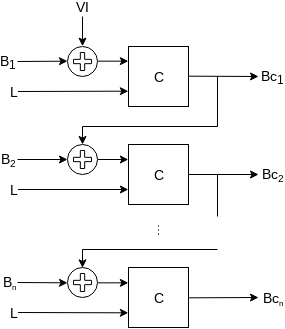
\includegraphics[width=0.7\linewidth]
            {contenidos/antecedentes/modos/diagramas/modo_cbc.png}
          \caption{Cifrado.}
      \end{center}
  \end{subfigure}
  \begin{subfigure}{0.45\textwidth}
      \begin{center}
          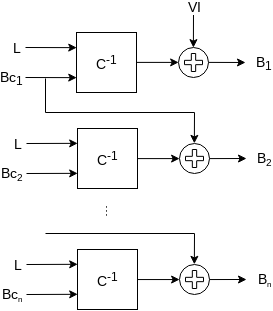
\includegraphics[width=0.7\linewidth]
            {contenidos/antecedentes/modos/diagramas/modo_cbc_inverso.png}
          \caption{Descifrado.}
      \end{center}
  \end{subfigure}
  \caption{Modo de operación CBC.}
  \label{figura:cbc}
\end{figure}

En la figura \ref{figura:cbc} se muestran los diagramas esquemáticos para
cifrar y descifrar; en los pseudocódigos \ref{cbc:1} y \ref{cbc:2} se muestran
unos de los posibles algoritmos a seguir. Es importante notar que mientras que
el proceso de cifrado debe ser forzosamente secuencial (por la dependencias
entre salidas), el proceso de descifrado puede ser ejecutado en paralelo.

\vspace{0.5cm}

% Látima que con los escapes en modo matemático dentro de los pseudocódigos
% se pierda totalmente la ventaja de trabajar con fuentes mono: por eso
% la alineación tan rara de los comentarios del próximo pseudocódigo.

\begin{pseudocodigo}[caption={Modo de operación CBC, cifrado.}, label={cbc:1}]
  entrada: llave $ L $; vector de inicialización $ VI $;
           bloques de mensaje $ B_1, B_2 \dots B_n $.
   salida: bloques de mensaje cifrado $ Bc_1, Bc_2 \dots Bc_n $.
  inicio
    $Bc_0$ $\gets$ $ VI $                         // El vector de incialización
    para_todo $B$                 // entra al primer bloque.
      $Bc_i$ $\gets$ C($L$, $B_i \oplus Bc_{i - 1}$)
    fin
    regresar $Bc$
  fin
\end{pseudocodigo}

\begin{pseudocodigo}[caption={Modo de operación CBC, descifrado.}, label={cbc:2}]
  entrada: llave $ L $; vector de inicialización $ VI $;
           bloques de mensaje cifrado $ Bc_1, Bc_2 \dots Bc_n $.
   salida: bloques de mensaje original $ B_1, B_2 \dots B_n $.
  inicio
    $Bc_0$ $\gets$ $ VI $
    para_todo $Bc$
      $B_i$ $\gets$ $C^{-1}$($L$, $Bc_i$) $\oplus$ $Bc_{i-1}$
    fin
    regresar $B$
  fin
\end{pseudocodigo}

%
% Modo de operación CFB, capítulo de antecedentes.
% Proyecto Lovelace.
%

\subsubsection{\textit{Cipher Feedback} (CFB)}

Al igual que la operación de cifrado de \gls{gl:cbc}, ambas operaciones
de \gls{gl:cfb} (cifrado y descifrado) están encadenadas bloque a bloque,
por lo que son de naturaleza secuencial. En este caso, lo que se cifra en el
primer paso es el \gls{gl:vector_de_inicializacion}; la salida de esto se opera
con un \verb|xor| sobre el primer bloque de texto en claro, para obtener el
primer bloque cifrado (figura \ref{fig:cfb}).

Esta distribución presenta varias ventajas con respecto a \gls{gl:cbc}:
las operaciones de cifrado y descifrado son sumamente similares, lo que permite
ser implementadas por un solo algoritmo (pseudocódigo \ref{cfb:1}); tanto para
cifrar como para descifrar solamente se ocupa la operación de cifrado del
algoritmo a bloques subyacente. Estas ventajas se deben principalmente a las
propiedades de la operación \verb|xor| (ecuación \ref{xor:inverso_igual}).

\begin{equation}
  \label{xor:inverso_igual}
  A \oplus B = C \quad \Rightarrow \quad A = B \oplus C
\end{equation}

\begin{figure}[H]
  \centering
  \begin{subfigure}{0.45\textwidth}
    \begin{center}
      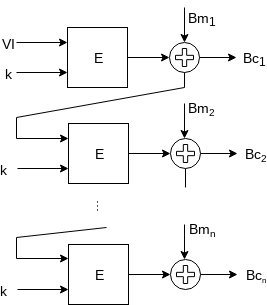
\includegraphics[width=0.6\linewidth]
        {contenidos/antecedentes/bloques/modos/diagramas/modo_cfb.png}
      \caption{Cifrado.}
    \end{center}
  \end{subfigure}
  \begin{subfigure}{0.45\textwidth}
    \begin{center}
      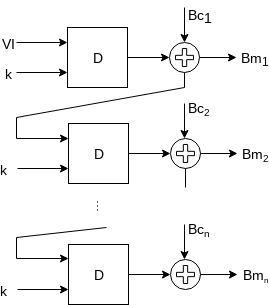
\includegraphics[width=0.6\linewidth]
        {contenidos/antecedentes/bloques/modos/diagramas/modo_cfb_inverso.png}
      \caption{Descifrado.}
    \end{center}
  \end{subfigure}
  \caption{\Gls{gl:modo_de_operacion} \gls{gl:cfb}.}
  \label{fig:cfb}
\end{figure}

\begin{pseudocodigo}[%
    caption={\Gls{gl:modo_de_operacion} \gls{gl:cfb}%
      (cifrado y descifrado).},
    label={cfb:1}%
  ]
  entrada: llave $ k $; vector de inicialización $ VI $;
           bloques de mensaje (cifrado o descifrado) $ Bm_1, Bm_2 \dots Bm_n $.
  salida:  bloques de mensaje (cifrado o descifrado) $ Bc_1, Bc_2 \dots Bc_n $.
  inicio
    $Bc_0$ $\gets$ $ VI $
    para_todo $Bm$
      $Bc_i$ $\gets$ $C_k$($Bc_{i - 1}$) $\oplus$ $Bm_i$
    fin
    regresar $Bc$
  fin
\end{pseudocodigo}

%
% Modo de operación OFB, capítulo de antecedentes.
% Proyecto Lovelace.
%

\newpage
\subsection{\textit{Output Feedback} (OFB)}

Este es muy similar al anterior (CFB), salvo porque la retroalimentación va
directamente de la salida del cifrador a bloques. De esta forma, nada que
tenga que ver con el texto en claro, llega al cifrado a bloques; este
solamente se la pasa cifrando una y otra vez el vector de inicialización.

\vspace{0.5cm}

\begin{figure}[H]
  \centering
  \begin{subfigure}{0.45\textwidth}
      \begin{center}
          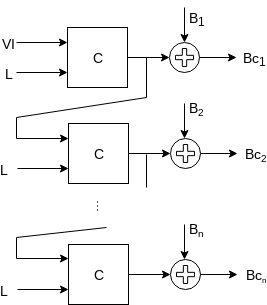
\includegraphics[width=0.7\linewidth]
            {contenidos/antecedentes/modos/diagramas/modo_ofb.png}
          \caption{Cifrado.}
      \end{center}
  \end{subfigure}
  \begin{subfigure}{0.45\textwidth}
      \begin{center}
          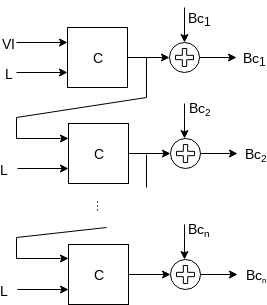
\includegraphics[width=0.7\linewidth]
            {contenidos/antecedentes/modos/diagramas/modo_ofb_inverso.png}
          \caption{Descifrado.}
      \end{center}
  \end{subfigure}
  \caption{Modo de operación OFB.}
\end{figure}

\begin{pseudocodigo}[caption={Modo de operación OFB (cifrado y descifrado).}]
  entrada: llave $ L $; vector de inicialización $ VI $;
           bloques de mensaje (cifrado o descifrado) $ B_1, B_2 \dots B_n $.
   salida: bloques de mensaje (cifrado o descifrado) $ Bc_1, Bc_2 \dots Bc_n $.
  inicio
    aux $\gets$ $ VI $
    para_todo $B$
      aux $\gets$ C($L$, aux)
      $Bc_i$ $\gets$  aux $\oplus$ $B_i$
    fin
    regresar $Bc$
  fin
\end{pseudocodigo}


